%%%%%%%%%%%%%%%%%%%%%%%%%%%%%%%%%%%%%%%%%%%%%%%%%%%%%%%%%%%%%%%%%%%%%%%%%%%%%%%%%%
\begin{frame}[fragile]\frametitle{}
\begin{center}
{\Large ChatGPT (Open AI)}
\end{center}
\end{frame}



%%%%%%%%%%%%%%%%%%%%%%%%%%%%%%%%%%%%%%%%%%%%%%%%%%%%%%%%%%%
\begin{frame}[fragile]\frametitle{Open AI}


\begin{itemize}
\item San Francisco-based artificial intelligence company
\item Famous for its well-known DALL·E, a deep-learning model that generates images from text instructions called prompts.
\item OpenAI Inc. is the non-profit parent company of the for-profit OpenAI LP.
\item Initially supported by Elon Musk
\item The CEO is Sam Altman, who previously was president of Y Combinator.
\item Microsoft is a partner and investor in the amount of \$1 billion dollars. They jointly developed the Azure AI Platform.
\item Mission: To ensure that artificial general intelligence benefits all of humanity
\item Prevent misuse of AI
\end{itemize}	 

\end{frame}

%%%%%%%%%%%%%%%%%%%%%%%%%%%%%%%%%%%%%%%%%%%%%%%%%%%%%%%%%%%
\begin{frame}[fragile]\frametitle{What is ChatGPT?}


\begin{itemize}
\item A Chatbot
\item Built by OpenAI
\item Released in Nov 2022
\item Got 1m users in 5 days  (Insta 2.5 months, Spotify 5m, Facebook 10m, Netflix 3.5yrs)
\end{itemize}	 

\end{frame}

%%%%%%%%%%%%%%%%%%%%%%%%%%%%%%%%%%%%%%%%%%%%%%%%%%%%%%%%%%%
\begin{frame}[fragile]\frametitle{What is ChatGPT?}


\begin{itemize}
\item GPT based
\item Trained on large amount of data
\item Gives answers like a human
\item Can ask Follow-up questions and even admit mistakes.
\end{itemize}	 

\end{frame}


%%%%%%%%%%%%%%%%%%%%%%%%%%%%%%%%%%%%%%%%%%%%%%%%%%%%%%%%%%%
\begin{frame}[fragile]\frametitle{GPTs Series}


\begin{itemize}
\item GPT + Generative Pre-trained Transformers
\item GPT-1, GPT-2 and GPT-3 are similar in terms of architecture 
\item Differ on the data and the number of transformer blocks with the number of incoming tokens.   
\item GPT-1 : 12 blocks, encoded using a Byte pair encoding, 512 tokens: 117 million parameters 
\item GPT-2 : 48 blocks, 1024 tokens: 1.5 billion parameters 
\item GPT-3 : 96 blocks, 2048 tokens: 175 billion parameters 
\end{itemize}	 

\end{frame}

%%%%%%%%%%%%%%%%%%%%%%%%%%%%%%%%%%%%%%%%%%%%%%%%%%%%%%%%%%%
\begin{frame}[fragile]\frametitle{GPTs Trainings}


\begin{itemize}
\item GPT-1 is trained in a self-supervised manner (learn to predict the next word in text data) and fine-tuned in a supervised learning manner. 
\item GPT-2 is trained in a fully self supervised way, focusing on zero-shot transfer
\item  GPT-3 is pre-trained in a self supervised manner exploring a bit more the few-shots fine-tuning.
\item GPT-1 is pre-trained on the BooksCorpus dataset, containing ~7000 books amounting to ~5GB of data
\item GPT-2 is pre-trained using the WebText dataset which is a more diverse set of internet data containing ~8M documents for about ~40 GB of data
\item GPT-3 uses an expanded version of the WebText dataset, two internet-based books corpora that are not disclosed and the English-language Wikipedia which constituted ~600 GB (45TB?) of data
\end{itemize}	 

\end{frame}



%%%%%%%%%%%%%%%%%%%%%%%%%%%%%%%%%%%%%%%%%%%%%%%%%%%%%%%%%%%
\begin{frame}[fragile]\frametitle{GPT 3.5 fine tuned = Chat GPT}


\begin{itemize}
\item GPT-3 was trained to predict the next word. Not much of context there.
\item Introducing prompting : provide with certain samples and context

\end{itemize}	 

			\begin{center}
			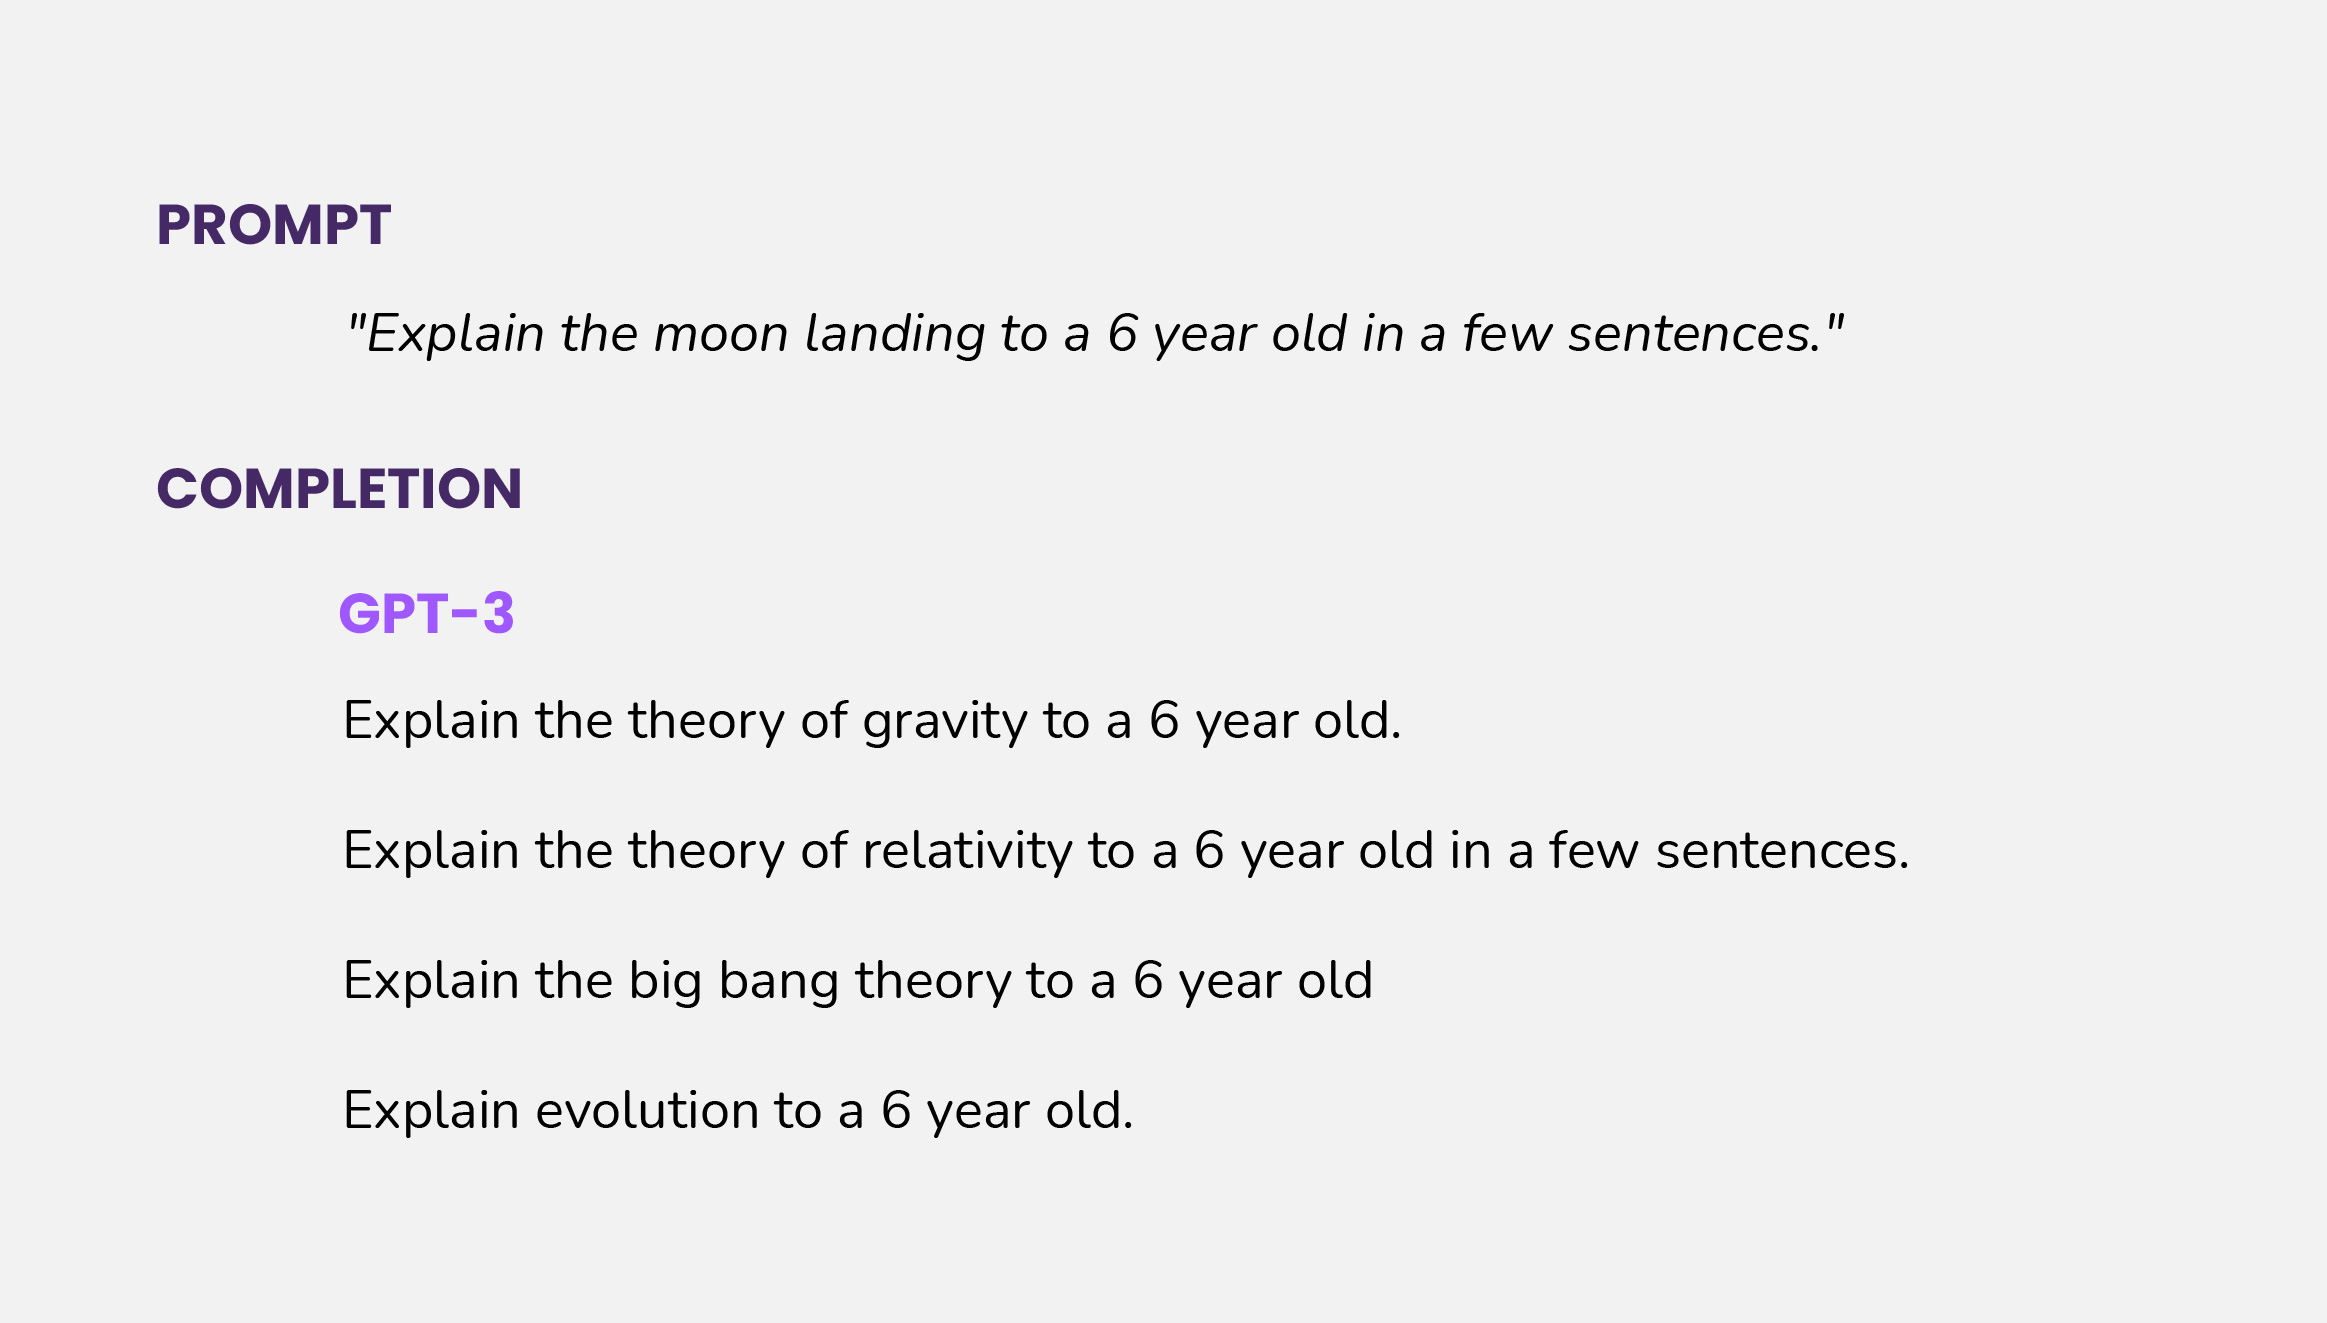
\includegraphics[width=0.6\linewidth,keepaspectratio]{chatgpt2}
			
			{\tiny "Example of misalignment between text to be predicted and final use"}
			\end{center}		
			
			
			{\tiny (Ref: ChatGPT: training process, advantages, and limitations - By Sergio Soage, Machine Learning Engineer at Aivo)}
			
\end{frame}

%%%%%%%%%%%%%%%%%%%%%%%%%%%%%%%%%%%%%%%%%%%%%%%%%%%%%%%%%%%
\begin{frame}[fragile]\frametitle{GPT 3.5 fine tuned = Chat GPT}


\begin{itemize}
\item To fix this misalignment, humans must be involved in teaching GPT, and in this way, GPT will be able to generate better questions as it evolves.
\end{itemize}	 

			\begin{center}
			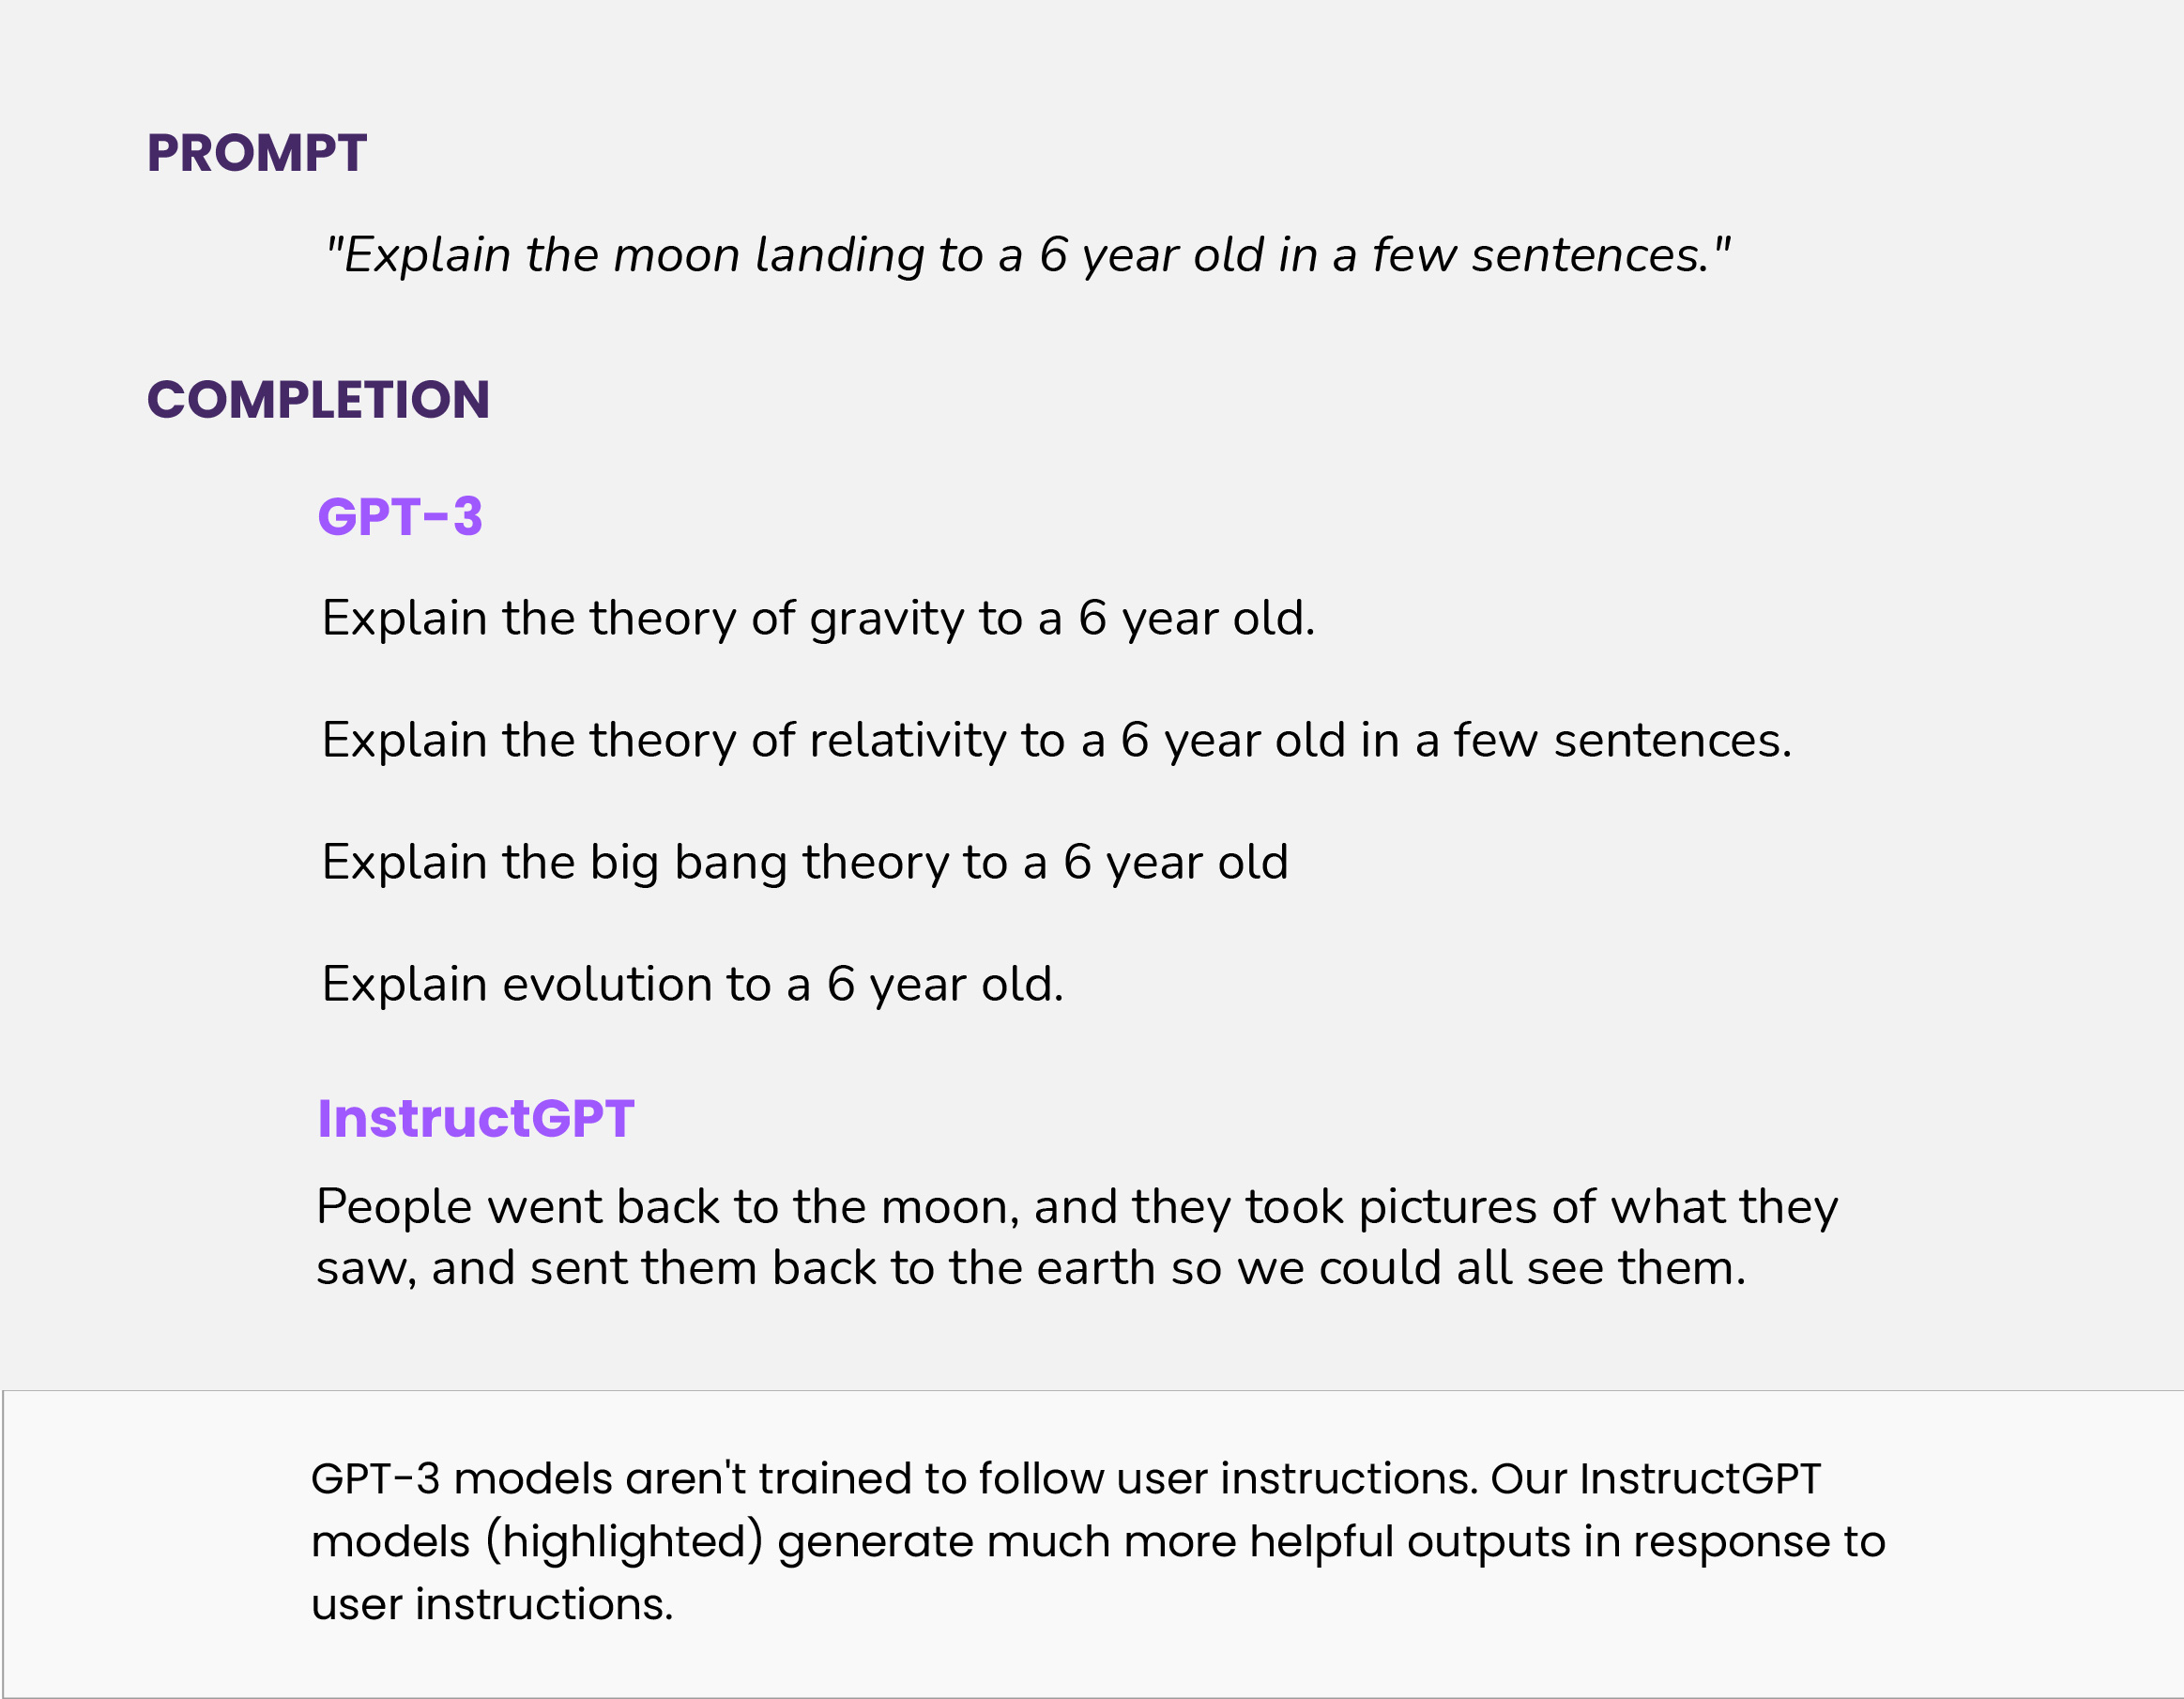
\includegraphics[width=0.6\linewidth,keepaspectratio]{chatgpt3}
			
			\end{center}		
			
			{\tiny (Ref: ChatGPT: training process, advantages, and limitations - By Sergio Soage, Machine Learning Engineer at Aivo)}
			
\end{frame}


%%%%%%%%%%%%%%%%%%%%%%%%%%%%%%%%%%%%%%%%%%%%%%%%%%%%%%%%%%%
\begin{frame}[fragile]\frametitle{GPT 3.5 fine tuned = Chat GPT}

\begin{itemize}
\item GPT-3.5 = Better of GPT-3 and sibling model InstructGPT + training(manually labeled data + reinforcement learning)
\item GPT-3.0’s answer is short and common but InstructGPT gives answers that the users prefer.
\end{itemize}	 
			\begin{center}
			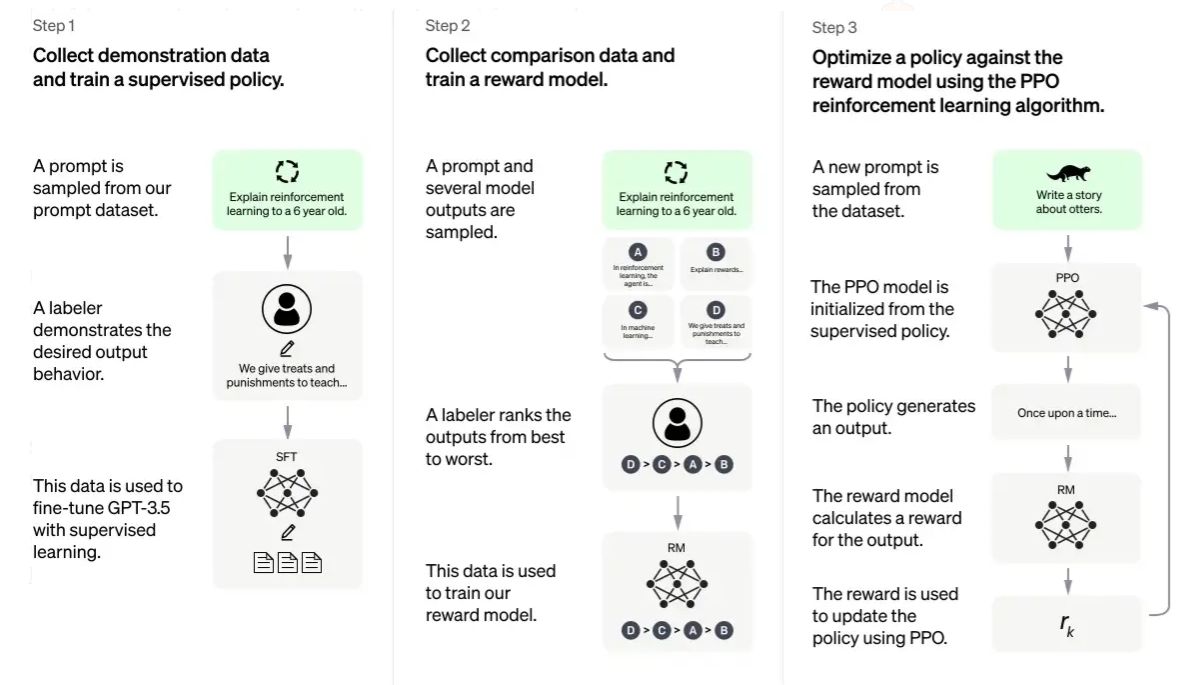
\includegraphics[width=\linewidth,keepaspectratio]{chatgpt1}
			\end{center}		
			
			\tiny{(Ref: https://openai.com/blog/chatgpt/)}
\end{frame}

%%%%%%%%%%%%%%%%%%%%%%%%%%%%%%%%%%%%%%%%%%%%%%%%%%%%%%%%%%%
\begin{frame}[fragile]\frametitle{Step 1}

\begin{itemize}
\item Have a prompts dataset 
\item Do fine-tuning using supervised learning. 
\item Simple but very expensive.
\end{itemize}	 

			\begin{center}
			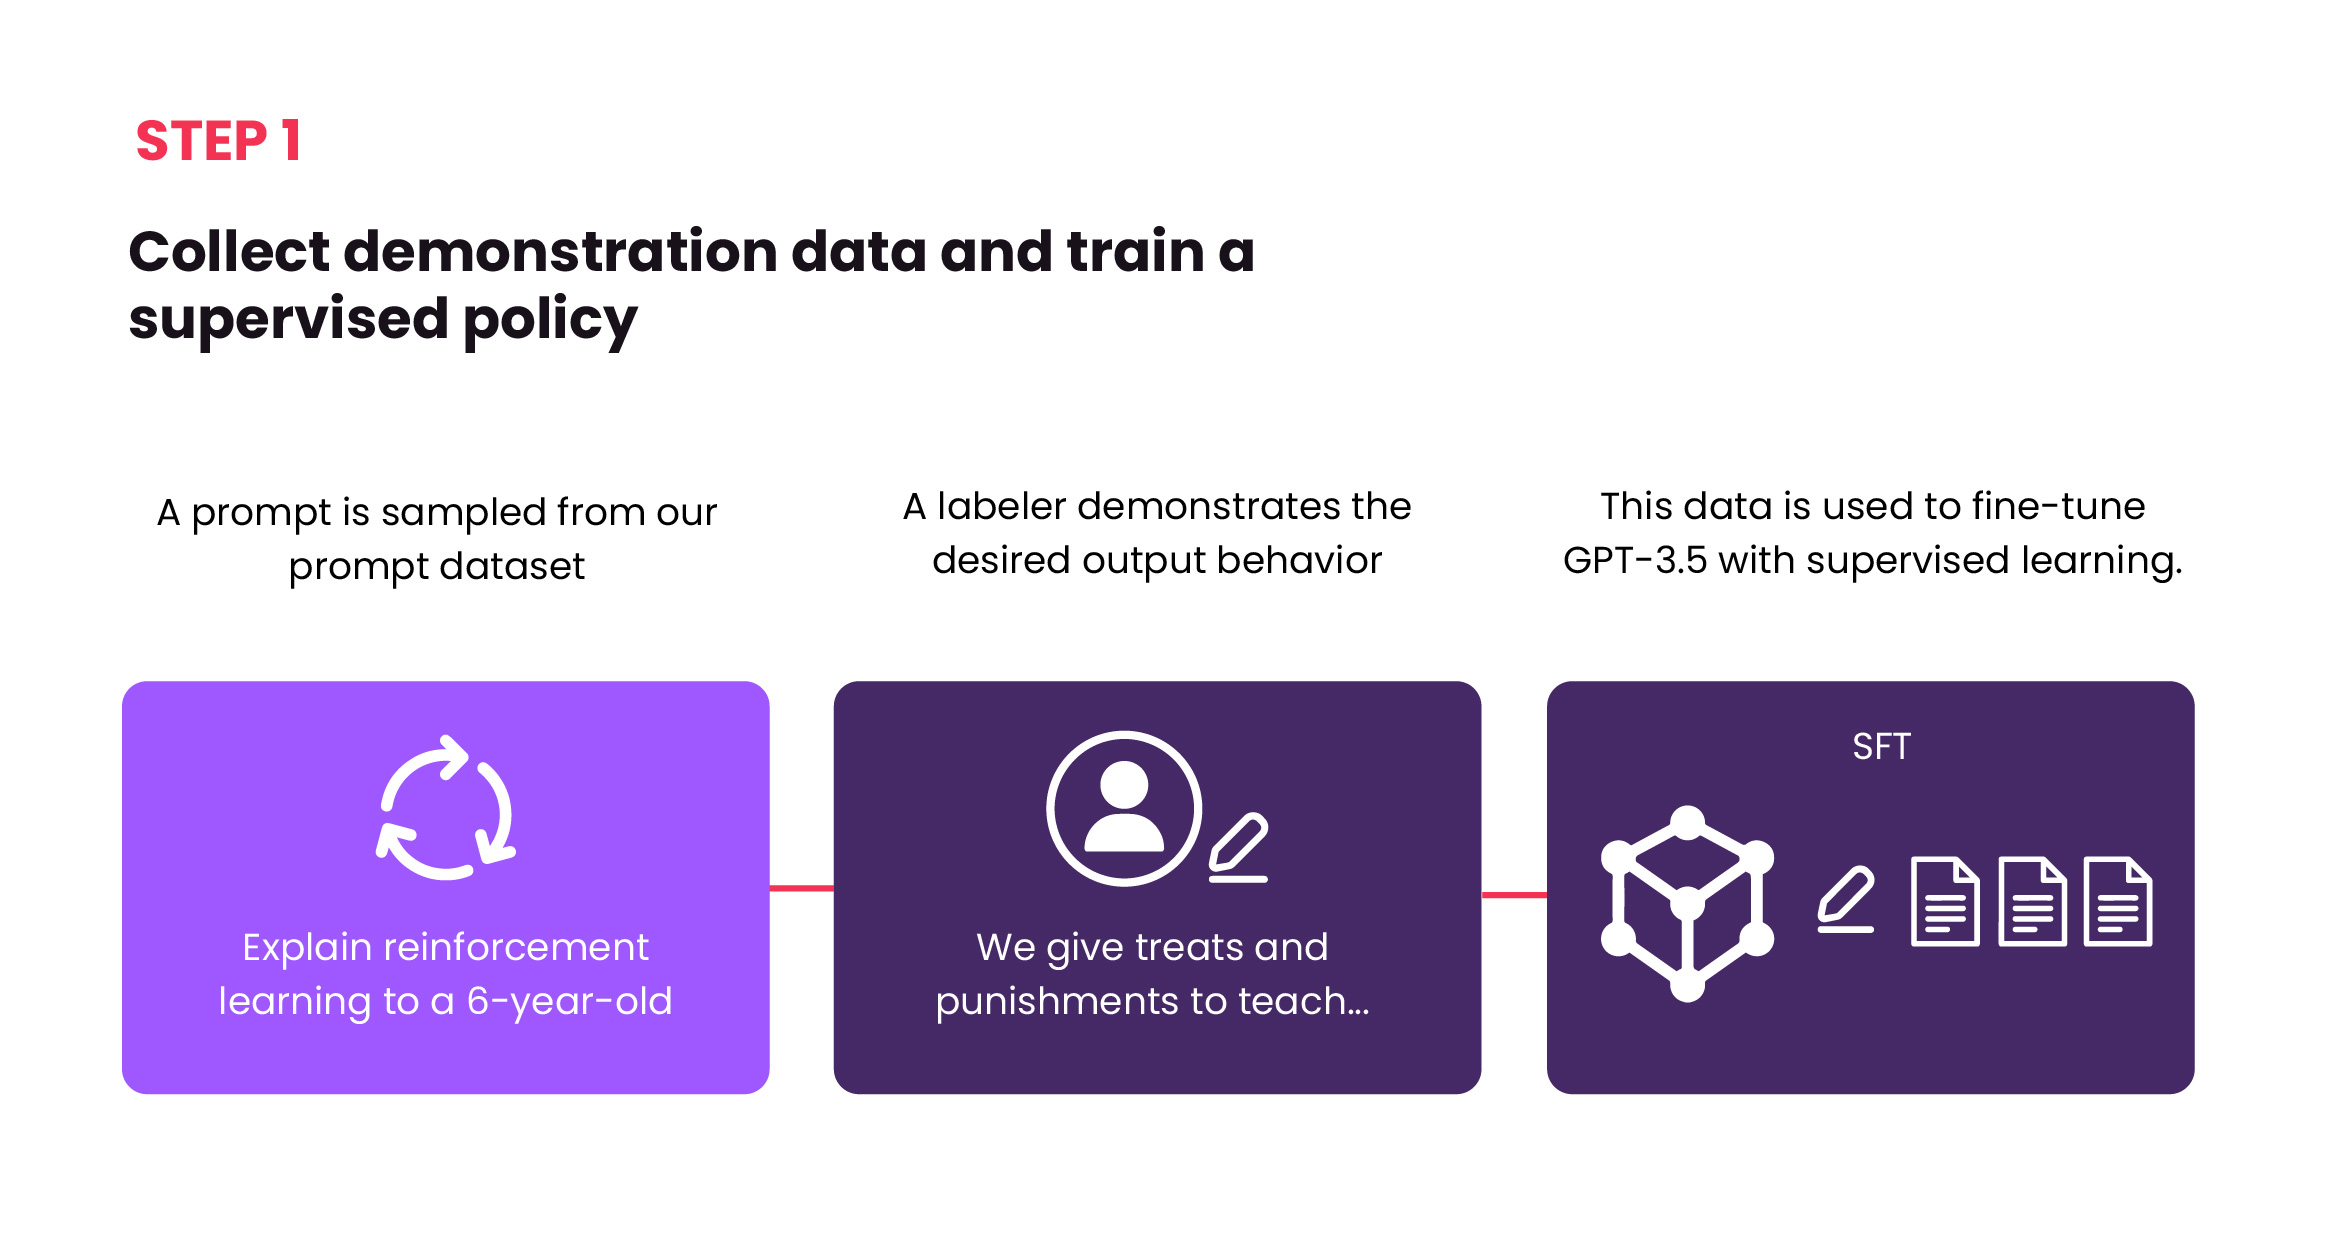
\includegraphics[width=0.6\linewidth,keepaspectratio]{chatgpt4}
			
			\end{center}		
			
			{\tiny (Ref: ChatGPT: training process, advantages, and limitations - By Sergio Soage, Machine Learning Engineer at Aivo)}
			
\end{frame}

%%%%%%%%%%%%%%%%%%%%%%%%%%%%%%%%%%%%%%%%%%%%%%%%%%%%%%%%%%%
\begin{frame}[fragile]\frametitle{Step 2}

\begin{itemize}
\item Human feedback provides a ranking of responses
\item Reinforcement Learning: which is "rewarded" and captures human preferences, reducing misalignment.
\end{itemize}	 

			\begin{center}
			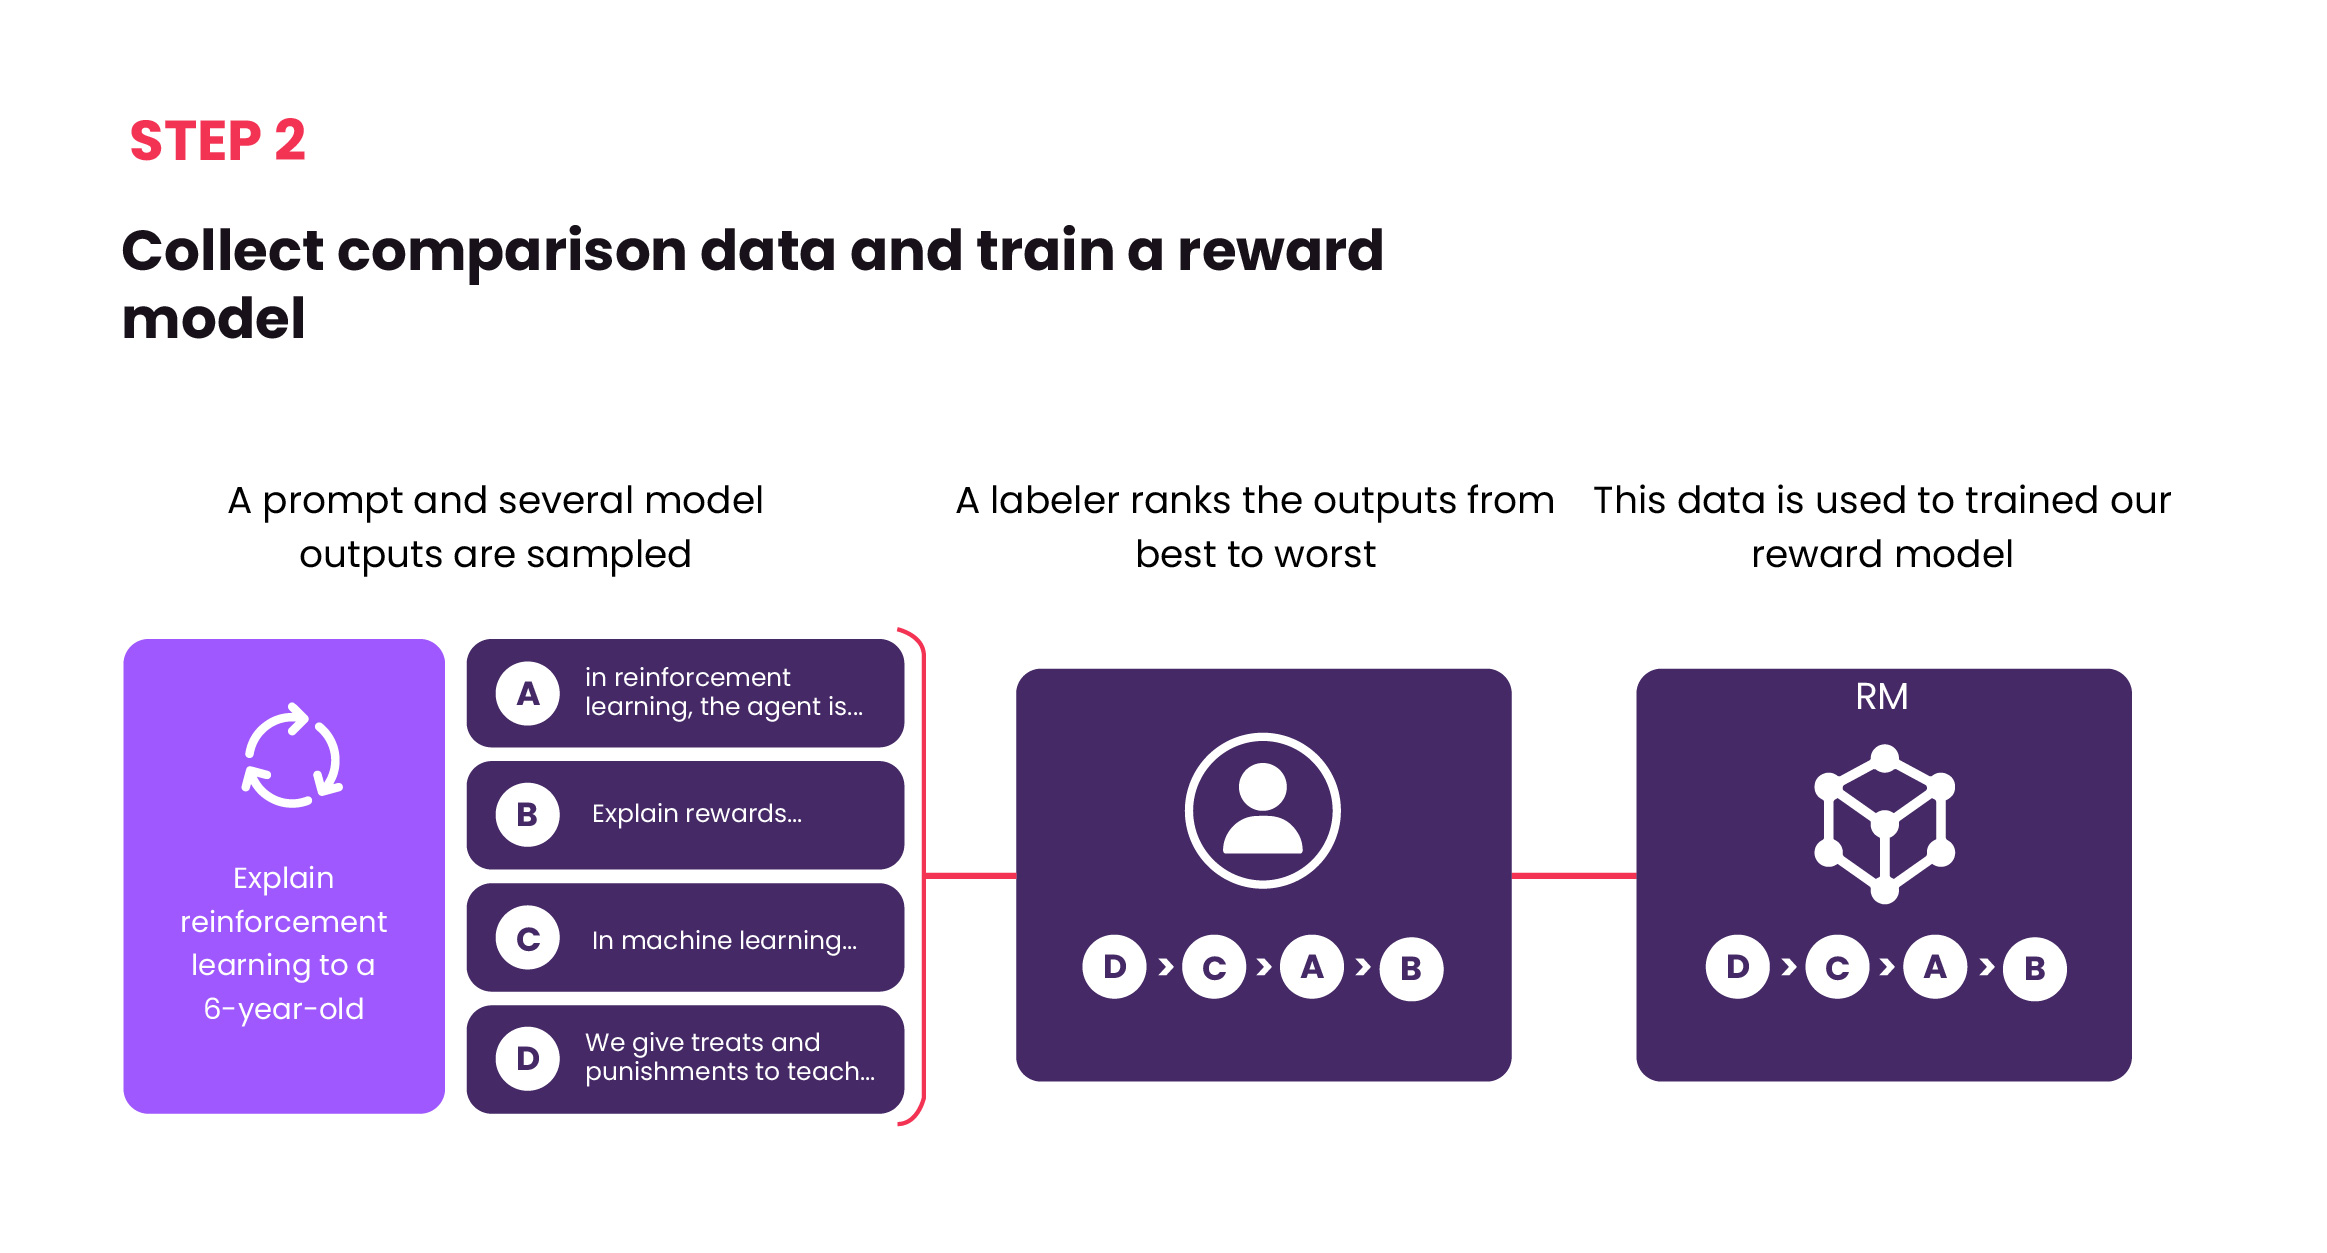
\includegraphics[width=0.6\linewidth,keepaspectratio]{chatgpt5}
			
			\end{center}		
			
			{\tiny (Ref: ChatGPT: training process, advantages, and limitations - By Sergio Soage, Machine Learning Engineer at Aivo)}
			
\end{frame}

%%%%%%%%%%%%%%%%%%%%%%%%%%%%%%%%%%%%%%%%%%%%%%%%%%%%%%%%%%%
\begin{frame}[fragile]\frametitle{Step 3}

\begin{itemize}
\item  Treat GPT as a ``policy'' (any function that returns a feasible action for a problem) and optimize it using RL against the learned reward.
\item PPO ( Proximal Policy Optimization, a policy gradient method) is used and, in this way, GPT is better aligned.
\end{itemize}	 

			\begin{center}
			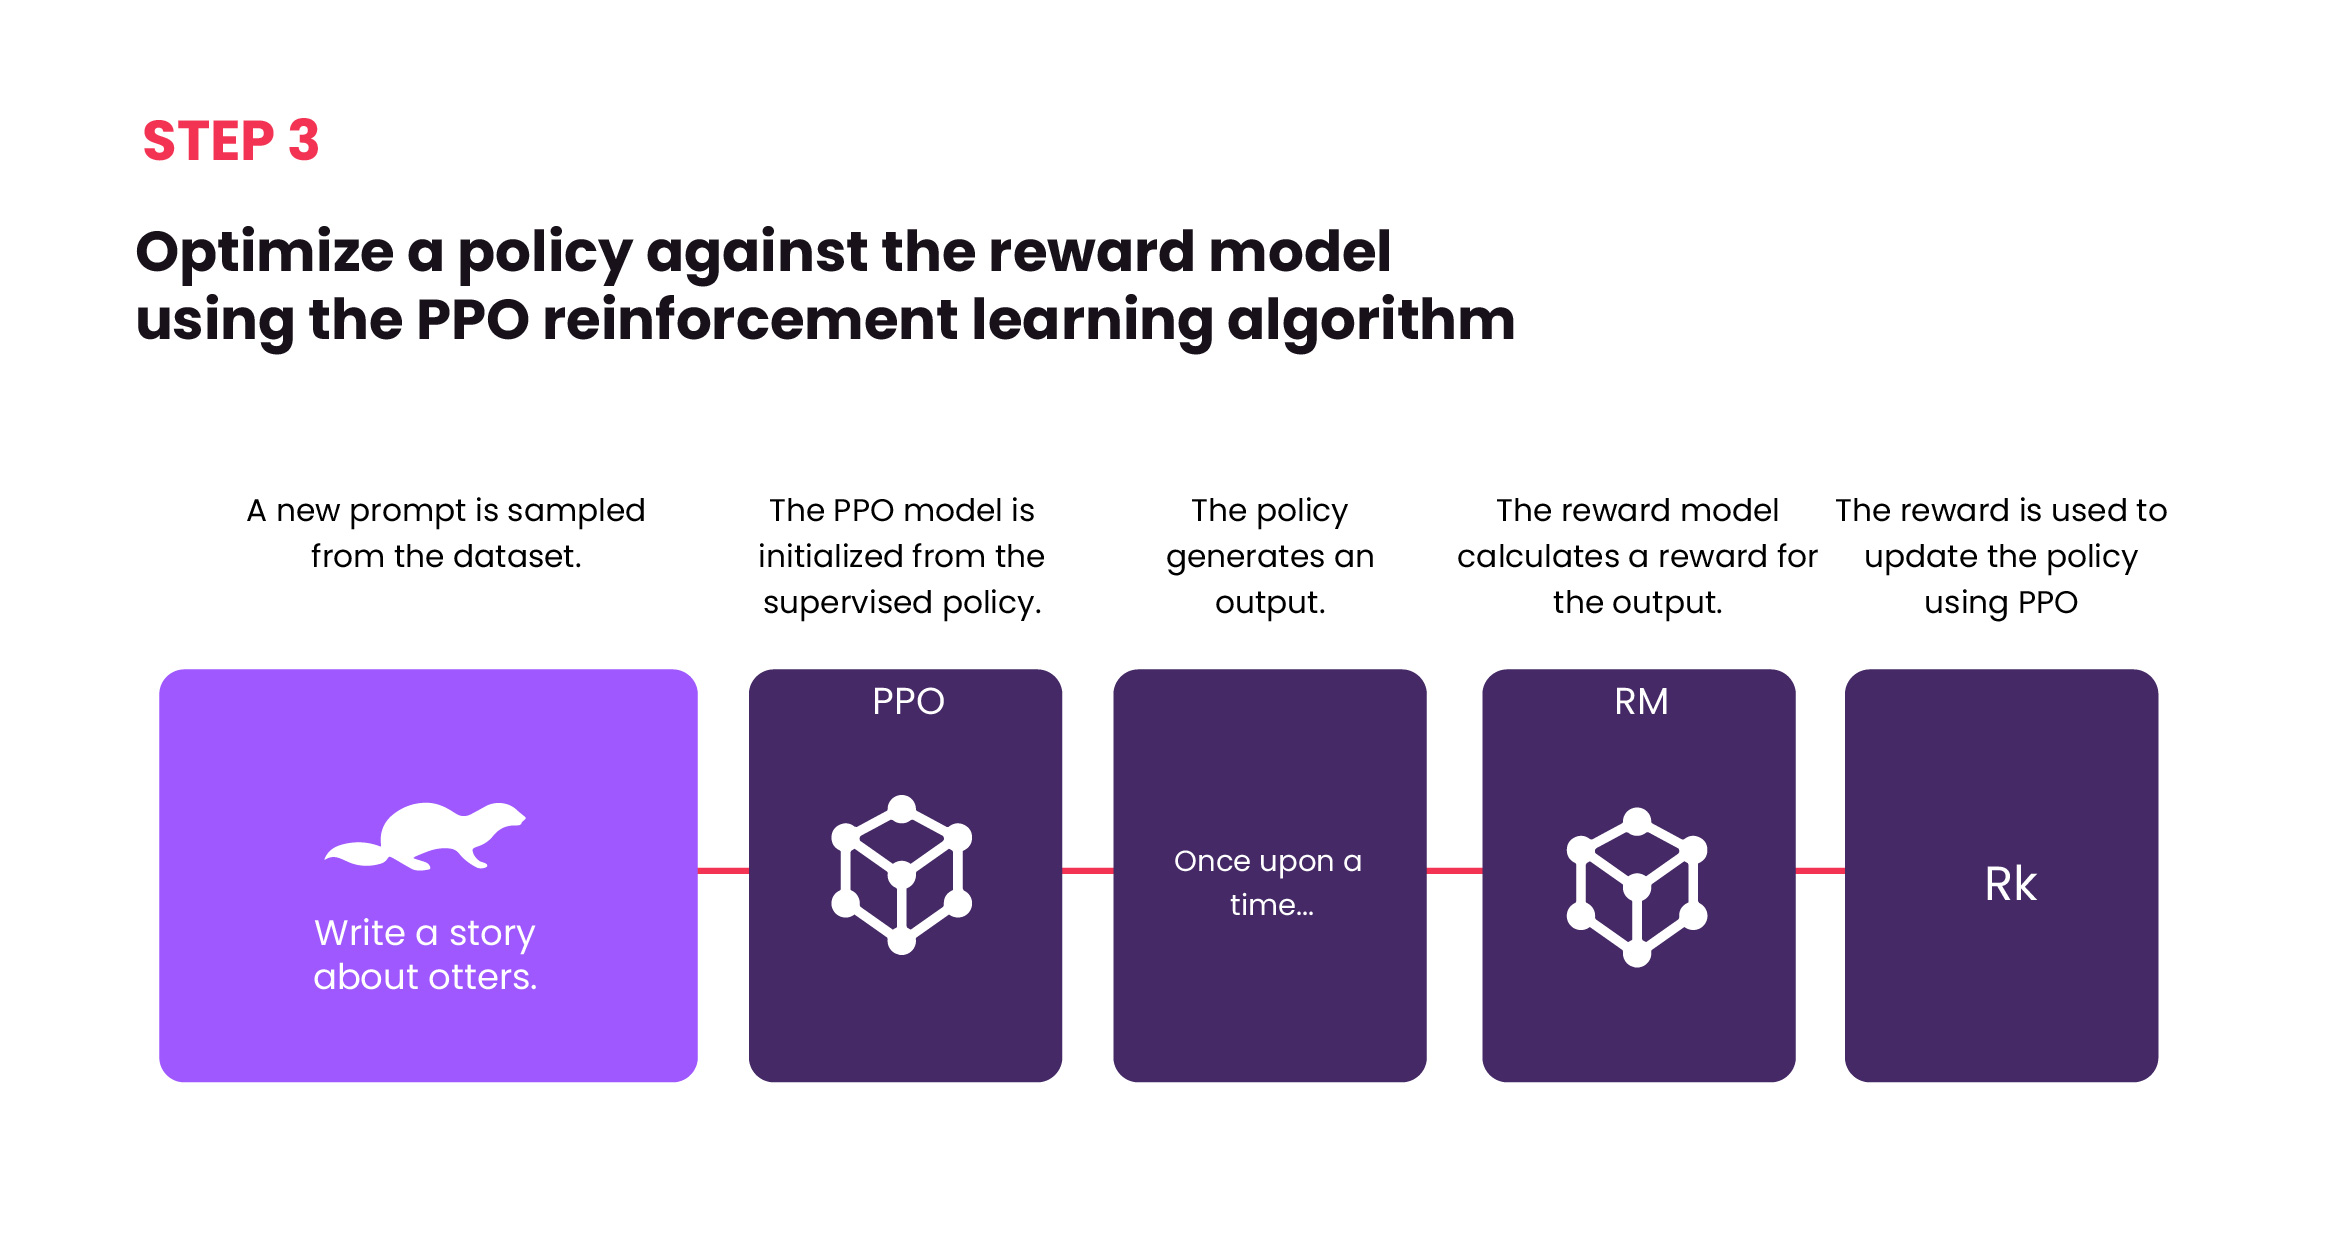
\includegraphics[width=0.6\linewidth,keepaspectratio]{chatgpt6}
			
			\end{center}		
			
			{\tiny (Ref: ChatGPT: training process, advantages, and limitations - By Sergio Soage, Machine Learning Engineer at Aivo)}
			
\end{frame}


%%%%%%%%%%%%%%%%%%%%%%%%%%%%%%%%%%%%%%%%%%%%%%%%%%%%%%%%%%%
\begin{frame}[fragile]\frametitle{Advantages}


\begin{itemize}
\item Creative Assistant, random-mix-ideas
\item Will replace mundane language tasks, How to articles, homeworks, etc
\item Supports more complex instructions, ``reasoning'' tasks
\end{itemize}	 

\end{frame}

%%%%%%%%%%%%%%%%%%%%%%%%%%%%%%%%%%%%%%%%%%%%%%%%%%%%%%%%%%%
\begin{frame}[fragile]\frametitle{Dis-advantages}


\begin{itemize}
\item Cannot replace humans for innovation, for which data does not exist already
\item Keeps ``hallucinating''
\item Tends to write plausible but incorrect content with confidence
\item Cannot get language structure right all the time, e.g try getting ghazal written
\end{itemize}	 

\end{frame}

%%%%%%%%%%%%%%%%%%%%%%%%%%%%%%%%%%%%%%%%%%%%%%%%%%%%%%%%%%%
\begin{frame}[fragile]\frametitle{Conclusion}



			\begin{center}
			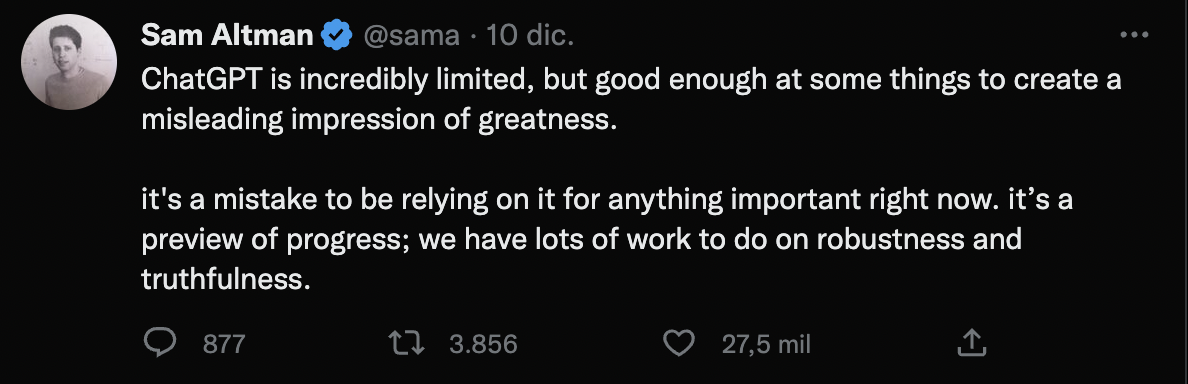
\includegraphics[width=\linewidth,keepaspectratio]{chatgpt7}
			
			\end{center}		
			
			{\tiny (Ref: ChatGPT: training process, advantages, and limitations - By Sergio Soage, Machine Learning Engineer at Aivo)}
			

\end{frame}